% SC4053 --- Chapter 5: Cryptography (Signatures, Merkle, Commitments) (0->100)
\chapter{Cryptography: Signatures, Merkle Trees and Commitments}\label{ch:crypto}

\begin{quote}
\emph{``Cryptography replaces the clerk who checks your signature with mathematics that anyone can verify but no one can forge.''} --- This chapter rebuilds that mathematics from hashes and discrete logs to Merkle proofs and hiding commitments.
\end{quote}

\noindent\fbox{\parbox{\dimexpr\linewidth-2\fboxsep-2\fboxrule}{%
\textbf{From zero: no crypto background assumed beyond Ch.~1 hashes.} We start from wax seals (authenticate, tamper-evident, non-repudiable) and translate each property into a hash/signature/commitment primitive, with definitions, examples and Python verifiers.}}
\vspace{0.4em}

\section*{Learning Outcomes}
After this chapter you will be able to:
\begin{enumerate}[label=(L\arabic*)]
    \item define digital signatures (Gen/Sign/Verify) and state EUF-CMA security;
    \item derive Ethereum addresses from ECDSA/secp256k1 keys and verify a transaction signature;
    \item construct a Merkle tree, prove inclusion in $O(\log n)$ and verify the proof;
    \item explain hash commitments (hide + bind) and Pedersen-style intuition;
    \item sketch zero-knowledge proof intuition and where ZK is used in blockchains.
\end{enumerate}

% ============================================================
\section{Digital Signatures: Seals that Mathematics Checks}\label{sec:sigs}
A \emph{digital signature scheme} is a triple $(\mathsf{Gen},\mathsf{Sign},\mathsf{Verify})$:
\begin{itemize}[leftmargin=1.2em]
    \item $\mathsf{Gen}()\to(sk,pk)$ random keypair.
    \item $\mathsf{Sign}(sk,m)\to\sigma$.
    \item $\mathsf{Verify}(pk,m,\sigma)\in\{0,1\}$.
\end{itemize}
Correctness: honest signatures verify. Security (EUF-CMA): without $sk$, no efficient adversary can forge a valid $\sigma$ on a new $m$, even after seeing signatures on chosen messages.

Blockchains use ECDSA on curve secp256k1 (Bitcoin/Ethereum) and increasingly Ed25519/schnorr. Intuition: $sk$ is a scalar $d$, $pk=dG$ (scalar multiplication of generator $G$); forging needs discrete log.

\begin{figure}[h]\centering
\begin{tikzpicture}[scale=0.84, every node/.style={font=\scriptsize},
  box/.style={draw,rounded corners=3pt,minimum width=1.95cm,minimum height=0.85cm,align=center,thick}]
\node[box,fill=blue!15] (gen) at (0,1.85) {Keygen\\ \tiny $d\!\xleftarrow{\$}\![1,n)$\\ $Q=dG$};
\node[box,fill=green!14] (sign) at (3.30,1.85) {Sign\\ \tiny $\sigma=(r,s)$\\ on $H(m)$};
\node[box,fill=orange!15] (ver) at (6.60,1.85) {Verify\\ \tiny check\\ $r,s$ vs $Q$};
\draw[->,thick,blue!60!black] (gen)--(sign) node[midway,above,font=\tiny] {$sk,pk$}; 
\draw[->,thick,green!50!black] (sign)--(ver) node[midway,above,font=\tiny] {$m,\sigma$};
\node[box,fill=yellow!16] (addr) at (6.60,0.55) {Address\\ \tiny $\text{keccak}(pk)[12:]$\\ last 20 bytes};
\draw[->,thick,orange!60!black,dashed] (ver)--(addr) node[midway,right,font=\tiny] {derive};
\node[font=\tiny,fill=blue!7,draw=gray!50,rounded corners=2pt,inner sep=1pt,align=center] at (3.30,0.55) {Ethereum: $m$ includes nonce, gas, to, value, data, chainId (EIP-155)\\Signature $(v,r,s)$ commits to all fields.};
% legend
\node[draw,fill=blue!15,minimum width=0.32cm,minimum height=0.18cm] at (0.10,-0.25) {}; \node[font=\tiny,anchor=west] at (0.35,-0.25) {secret};
\node[draw,fill=green!14,minimum width=0.32cm,minimum height=0.18cm] at (1.55,-0.25) {}; \node[font=\tiny,anchor=west] at (1.80,-0.25) {public};
\node[draw,fill=orange!15,minimum width=0.32cm,minimum height=0.18cm] at (2.85,-0.25) {}; \node[font=\tiny,anchor=west] at (3.10,-0.25) {verify};
\end{tikzpicture}
\caption{ECDSA lifecycle: key generation $\to$ signing the hash of $m$ $\to$ verification with $pk$ $\to$ address derivation. Only $sk$ can produce a valid $(r,s)$, but anyone with $pk$ can check.}
\label{fig:ecdsa}
\end{figure}

\begin{lstlisting}[language=Python]
# ECDSA sign/verify demo (uses ecdsa lib; pip install ecdsa)
import hashlib, ecdsa
sk = ecdsa.SigningKey.generate(curve=ecdsa.SECP256k1)
vk = sk.verifying_key
msg = b"send 10 coins to Bob, nonce=4, chain=1"
sig = sk.sign(msg, hashfunc=hashlib.sha256)
print("verify:", vk.verify(sig, msg, hashfunc=hashlib.sha256))
# Ethereum address = keccak(pubkey)[-20:]
pub_bytes = b"\x04" + vk.to_string()  # uncompressed
# for demo, sha3 ~ keccak; use pysha3's keccak_256 in production
import hashlib
addr = hashlib.sha3_256(pub_bytes).hexdigest()[-40:]
print("addr 0x"+addr[:10]+"...")
# forge attempt with different key fails
sk2 = ecdsa.SigningKey.generate(curve=ecdsa.SECP256k1)
try: print("forge:", sk2.verifying_key.verify(sig, msg, hashfunc=hashlib.sha256))
except ecdsa.BadSignatureError: print("forge rejected")
\end{lstlisting}

% ============================================================
\section{Merkle Trees: One Hash Commits to Many}\label{sec:merkle}
A \emph{Merkle tree} hashes pairs recursively: leaves are $H(tx_i)$, internal node $H(left\parallel right)$, root $M$ commits to the whole set.

\begin{definition}[Merkle proof]\label{def:merkle-proof}
For $n=2^k$ leaves, a proof for $tx_i$ is the $k$ sibling hashes on the path to the root. Verification recomputes the root from $tx_i$ plus siblings and compares to $M$. Cost $O(\log n)$ hashes vs $O(n)$ to hash everything.
\end{definition}

\begin{figure}[h]\centering
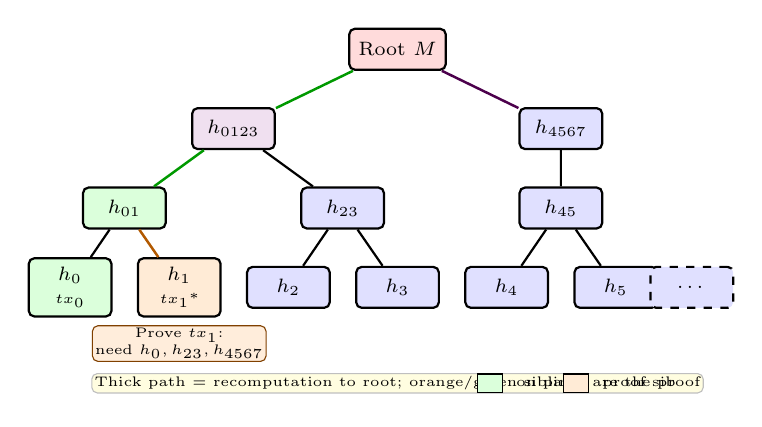
\begin{tikzpicture}[scale=0.84, every node/.style={font=\scriptsize},
  leaf/.style={draw,rounded corners=2pt,minimum width=1.05cm,minimum height=0.52cm,align=center,thick},
  node/.style={draw,rounded corners=2pt,minimum width=1.05cm,minimum height=0.52cm,align=center,thick}]
% leaves
\node[leaf,fill=green!14] (l0) at (0,0) {$h_0$\\ \tiny $tx_0$};
\node[leaf,fill=orange!16] (l1) at (1.65,0) {$h_1$\\ \tiny $tx_1$*};
\node[leaf,fill=blue!12] (l2) at (3.30,0) {$h_2$};
\node[leaf,fill=blue!12] (l3) at (4.95,0) {$h_3$};
\node[leaf,fill=blue!12] (l4) at (6.60,0) {$h_4$};
\node[leaf,fill=blue!12] (l5) at (8.25,0) {$h_5$};
\node[leaf,fill=blue!12,dashed] (l6) at (9.40,0) {\dots};
% level 1
\node[node,fill=green!14] (n01) at (0.82,1.20) {$h_{01}$};
\node[node,fill=blue!12] (n23) at (4.12,1.20) {$h_{23}$};
\node[node,fill=blue!12] (n45) at (7.42,1.20) {$h_{45}$};
% level 2
\node[node,fill=violet!12] (n0123) at (2.47,2.40) {$h_{0123}$};
\node[node,fill=blue!12] (n4567) at (7.42,2.40) {$h_{4567}$};
% root
\node[node,fill=red!14] (root) at (4.95,3.60) {Root $M$};
\draw[thick] (l0)--(n01); \draw[thick,orange!70!black,line width=0.9pt] (l1)--(n01);
\draw[thick] (l2)--(n23); \draw[thick] (l3)--(n23);
\draw[thick] (l4)--(n45); \draw[thick] (l5)--(n45);
\draw[thick,green!60!black,line width=0.9pt] (n01)--(n0123); \draw[thick] (n23)--(n0123);
\draw[thick] (n45)--(n4567);
\draw[thick,green!60!black,line width=0.9pt] (n0123)--(root); \draw[thick,violet!60!black,line width=0.9pt] (n4567)--(root);
% proof highlight
\node[font=\tiny,fill=orange!14,draw=orange!50!black,rounded corners=2pt,inner sep=1pt,align=center] at (1.65,-0.85) {Prove $tx_1$:\\need $h_0,h_{23},h_{4567}$};
\node[font=\tiny,fill=yellow!12,draw=gray!50,rounded corners=2pt,inner sep=1pt] at (4.95,-1.45) {Thick path = recomputation to root; orange/green siblings are the proof};
% legend
\node[draw,fill=green!14,minimum width=0.32cm,minimum height=0.18cm] at (6.35,-1.45) {}; \node[font=\tiny,anchor=west] at (6.60,-1.45) {on path};
\node[draw,fill=orange!16,minimum width=0.32cm,minimum height=0.18cm] at (7.65,-1.45) {}; \node[font=\tiny,anchor=west] at (7.90,-1.45) {proof sib};
\end{tikzpicture}
\caption{Merkle tree and inclusion proof: to prove $tx_1$ is in the block, reveal only 3 sibling hashes (not all $n$ leaves); verifier recomputes the thick path to the root $M$ stored in the header.}
\label{fig:merkle}
\end{figure}

\begin{lstlisting}[language=Python]
import hashlib
def H(x): return hashlib.sha256(x).hexdigest()
def merkle_root(leaves):
    layer = [H(l.encode()) for l in leaves]
    while len(layer) > 1:
        nxt = []
        for i in range(0, len(layer), 2):
            a, b = layer[i], layer[i+1] if i+1 < len(layer) else layer[i]
            nxt.append(H((a+b).encode()))
        layer = nxt
    return layer[0]
def merkle_proof(leaves, idx):
    # return sibling hashes along path
    layer = [H(l.encode()) for l in leaves]
    proof = []
    i = idx
    while len(layer) > 1:
        sib = i ^ 1
        if sib < len(layer): proof.append(layer[sib])
        # build next layer
        nxt=[]
        for j in range(0,len(layer),2):
            a,b = layer[j], layer[j+1] if j+1<len(layer) else layer[j]
            nxt.append(H((a+b).encode()))
        layer=nxt; i//=2
    return proof

leaves = [f"tx{i}" for i in range(8)]
root = merkle_root(leaves)
print("root", root[:12]+"...", "proof for tx1", [p[:8] for p in merkle_proof(leaves,1)])
\end{lstlisting}

% ============================================================
\section{Commitments and Zero-Knowledge Intuition}\label{sec:commit}
A \emph{commitment} $C=\mathsf{Commit}(m;r)$ hides $m$ (hiding) and binds to it (cannot open to $m'\ne m$). Simplest: $C=H(m\parallel r)$ with random $r$; open by revealing $(m,r)$. Blockchains use commitments for sealed-bid auctions, voting and light-client bridges. A fancier variant, Pedersen $C=g^m h^r$, is additively homomorphic.

\emph{Zero-knowledge proofs} prove ``I know $w$ with $P(w)=1$'' without revealing $w$. Intuition: prover and verifier play a game where a cheating prover would fail a random challenge with high probability, while an honest prover always passes and leaks nothing beyond the statement's truth. ZK-rollups (Ch.~6) use this to prove ``this batch of $1000$ transactions was executed correctly'' with a single short proof.

\begin{figure}[h]\centering
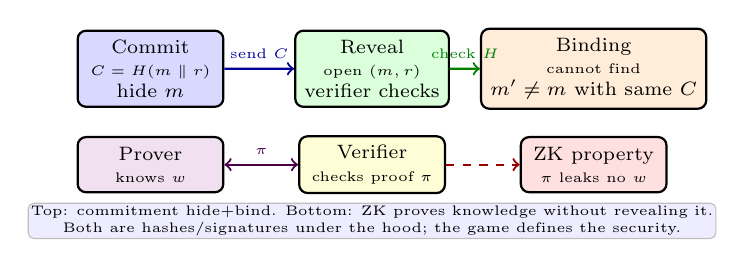
\begin{tikzpicture}[scale=0.84, every node/.style={font=\scriptsize},
  box/.style={draw,rounded corners=3pt,minimum width=1.85cm,minimum height=0.70cm,align=center,thick}]
\node[box,fill=blue!15] (commit) at (0,1.70) {Commit\\ \tiny $C=H(m\parallel r)$\\ hide $m$};
\node[box,fill=green!14] (reveal) at (3.35,1.70) {Reveal\\ \tiny open $(m,r)$\\ verifier checks};
\node[box,fill=orange!15] (bind) at (6.70,1.70) {Binding\\ \tiny cannot find\\ $m'\ne m$ with same $C$};
\draw[->,thick,blue!60!black] (commit)--(reveal) node[midway,above,font=\tiny] {send $C$};
\draw[->,thick,green!50!black] (reveal)--(bind) node[midway,above,font=\tiny] {check $H$};
\node[box,fill=violet!12] (prover) at (0,0.25) {Prover\\ \tiny knows $w$};
\node[box,fill=yellow!16] (verif) at (3.35,0.25) {Verifier\\ \tiny checks proof $\pi$};
\node[box,fill=red!12] (zk) at (6.70,0.25) {ZK property\\ \tiny $\pi$ leaks no $w$};
\draw[<->,thick,violet!60!black] (prover)--(verif) node[midway,above,font=\tiny] {$\pi$};
\draw[->,thick,red!60!black,dashed] (verif)--(zk);
\node[font=\tiny,fill=blue!7,draw=gray!50,rounded corners=2pt,inner sep=1pt,align=center] at (3.35,-0.60) {Top: commitment hide+bind. Bottom: ZK proves knowledge without revealing it.\\Both are hashes/signatures under the hood; the game defines the security.};
\end{tikzpicture}
\caption{Commitment lifecycle (top) and ZK intuition (bottom). Commitments appear in sealed auctions and state channels; ZK proofs compress verification (Ch.~6).}
\label{fig:commit-zk}
\end{figure}

\begin{example}[Sealed-bid auction]\label{ex:sealed}
Bidders commit $C_i=H(bid_i\parallel r_i)$ on-chain. After the deadline they reveal. No one can change $bid_i$ after seeing others (binding) and no one learns bids before the reveal (hiding). A ZK variant can prove ``my bid is highest'' without revealing the amount.
\end{example}

\begin{remark}[Hash-then-sign and domain separation]\label{rem:hash-sign}
We never sign the raw message $m$ (which may be huge); we sign $H(m)$. Collision resistance of $H$ ensures signing $H(m)$ is as secure as signing $m$, while keeping signatures constant size. EIP-712 adds \emph{domain separation} (chainId, contract address) into that hash so a signature for one dApp cannot be replayed in another -- the same replay protection we saw in Ch.~3, now at the crypto layer.
\end{remark}

\begin{example}[Merkle in the wild]\label{ex:merkle-wild}
Bitcoin's block header commits to all transactions via one Merkle root; Ethereum's state uses a Merkle-Patricia trie so a single 32-byte state root commits to every account, storage slot and code hash. Light clients download only headers and request Merkle/MPT proofs for the keys they care about.
\end{example}

% ============================================================
\section{Exercises}\label{sec:ch05-exercises}
\begin{enumerate}[label=E5.\arabic*, leftmargin=*, itemsep=0.6em]
    \item \textbf{Sign/verify by hand.} Given toy parameters $G,n$ small, compute $\mathsf{Sign}$ and $\mathsf{Verify}$ on a short message. Show that flipping one bit of the message fails verification.
    \item \textbf{Merkle drill.} Build a tree for 8 leaves. Give the proof for leaf 5 (list siblings in order), recompute the root, and show what changes if leaf 2 is tampered.
    \item \textbf{Light client.} A header stores root $M$. Explain step-by-step how a light client with only $M$ verifies that $tx$ is in the block using $O(\log n)$ hashes. Why is storing $M$ enough?
    \item \textbf{Commit game.} Alice commits $H(m\parallel r)$ with 128-bit $r$. Argue hiding against a brute-force adversary and binding against a collision finder. When does $H(m)$ alone fail to hide?
    \item \textbf{ZK intuition.} State a statement you would ZK-prove in a rollup (e.g., ``batch root is correct''). Who is prover/verifier, what is the witness, and why does the verifier not need to re-execute all transactions?
\end{enumerate}

\section*{Chapter Notes}
Katz--Lindell, Ch.~12-13 for signatures and hash commitments; Boneh--Shoup for pairing-based ZK; Nakamoto (2008) and Wood (Yellow Paper) for Merkle roots in headers; Ben-Sasson et al., ``Zerocash'' (2014) and Groth16 (2016) for the ZK lineage leading to ZK-rollups. Antonopoulos Ch.~4-6 is a practical companion for keys/addresses.
% End Ch05
